\documentclass{article}
\usepackage[T1]{fontenc}
\usepackage[utf8]{inputenc}
\usepackage[english, icelandic]{babel}
\usepackage{amsmath}
\usepackage{amssymb}
\usepackage{amsthm}
\usepackage{gensymb}
\usepackage{parskip}
\usepackage{mathtools}
\usepackage{xfrac}
\usepackage{graphicx}
\usepackage{xcolor}
\usepackage{tikz}
\usetikzlibrary{calc}
\usepackage{verbatim}
\usepackage{minted}
\usepackage{multicol}
\parskip 0pt

\DeclareMathOperator{\lcm}{lcm}
\DeclareMathOperator{\diam}{diam}
\DeclareMathOperator{\dist}{dist}
\DeclareMathOperator{\ord}{ord}
\DeclareMathOperator{\Aut}{Aut}
\DeclareMathOperator{\Inn}{Inn}
\DeclareMathOperator{\Ker}{Ker}
\DeclareMathOperator{\trace}{trace}
\DeclareMathOperator{\fix}{fix}
\newcommand\floor[1]{\left\lfloor#1\right\rfloor}
\newcommand\ceil[1]{\left\lceil#1\right\rceil}
\newcommand\abs[1]{\left|#1\right|}
\newcommand\p[1]{\left(#1\right)}
\newcommand\sqp[1]{\left[#1\right]}
\newcommand\cp[1]{\left\{#1\right\}}
\newcommand\norm[1]{\left\lVert#1\right\rVert}
\renewcommand\qedsymbol{$\blacksquare$}

\pagenumbering{gobble}

\graphicspath{{myndir/}}

\begin{document}

\begin{titlepage}
	\centering
	{\scshape\LARGE Háskóli Íslands \par}
	\vspace{1cm}
	{\scshape\Large Töluleg greining \par}
	\vspace{1.5cm}
	{\huge\bfseries Stórt Verkefni II \par}
	\vspace{2cm}
	{\Large\itshape Atli Fannar Franklín \\ Hjörvar Logi Ingvarsson \par}
	\vfill
	Kennari: \par
	Sigurður Freyr Hafstein \par 

	\vfill

	{\large \today\par}
\end{titlepage}

Við munum eins og síðast nota sage í þessu verkefni. Sage er python með fullt af aukapökkum á við numpy, scipy, sympy og fleira. Þar sem síðasti liðurinn biður um að gera þetta fyrir almennar kúrvur munum við gera það frá byrjun. Við gerum þá ráð fyrir að við fáum föllin $x, y, x', y'$ gefin. Við verðum einnig að gera ráð fyrir að $x, y, x', y'$ hagi sér 'ágætlega vel' til þess að fá tölulega nákvæmni í svari, en meir um það síðar. Fyrsta liðinn má gera með eftirfarandi hætti (tol er tolerance-inn): \\

\begin{minted}{python}
def adaptquad(f, ac, bc, t, ao, bo):
    def appr(x, y):
        return (y - x) * (f(x) + f(y)) / 2
    c = (ac + bc) / 2
    sab = appr(ac, bc)
    sac = appr(ac, c)
    sbc = appr(c, bc)
    ct = 3 * t * (bc - ac) / (bo - ao)
    if abs(sab - sac - sbc) < ct:
        return sac + sbc
    else:
        s1 = adaptquad(f, ac, c, t, ao, bo)
        s2 = adaptquad(f, c, bc, t, ao, bo)
        return s1 + s2

def arclen(dx, dy, T, tol):
    def f(x):
        return sqrt(dx(x) ** 2 + dy(x) ** 2)
    return adaptquad(f, 0, T, tol, 0, T)
\end{minted}

\vspace*{0.5cm}

Ef við skoðum svo lið 2 þá eigum við fyrir gefið $s \in [0, 1]$ að ákvarða $t^*(s)$ þ.a. 

\[\frac{\int_0^{t^*(s)} \sqrt{x'(t)^2 + y'(t)^2}dt}{\int_0^1 \sqrt{x'(t)^2 + y'(t)^2}dt} = s\]

Til þess að getað helmingunarleitað að núllstöð endurritum við þetta sem

\[\int_0^{t^*(s)} \sqrt{x'(t)^2 + y'(t)^2}dt - s\int_0^1 \sqrt{x'(t)^2 + y'(t)^2}dt = 0\]

Við viljum nú ákvarða $t^*(s)$ upp að einhverjum gefnum tolerance $r$. Hins vegar þar sem $c$ er hvaða fall sem er frá $[0, 1]$ í $[0, 1]$ getur $c'$ hagað sér afar illa. Það þýðir að tolerance-inn okkar getur orðið enginn nema við reiknum heildið upp að miklu meiri nákvæmni en $r$. En þar sem að reikna tolerance-inn sem þarf fyrir hvaða $c$ sem er er afar flókið leyfði Sigurður Freyr Hafstein okkur að sleppa því. Því reiknum við heildið bara upp að tolerance $r$, en munum samt að þetta gæti gefið okkur minni en $r$ tolerance í lokasvari fyrir leiðinleg $c$. Með þetta allt í huga fáum við eftirfarandi forrit: \\

\begin{minted}{python}
def bissearch(dx, dy, tol, s, c):
    alen = arclen(dx, dy, 1, tol)
    def f(x):
        return arclen(dx, dy, x, tol) - c(s) * alen
    lo, hi = 0, 1
    while hi - lo >= tol:
        mid = (hi + lo) / 2
        if f(mid) < 0:
            lo = mid
        else:
            hi = mid
    return (hi + lo) / 2
\end{minted}

\vspace*{0.5cm}

Nú til þess að gera allt sem er beðið um fyrir öll progress curve-in gefin í síðasta lið skigreinum við eftirfarandi föll og breytur: \\

\begin{minted}{python}
def px(t):
    return 0.5 + 0.3 * t + 3.9 * t ** 2 - 4.7 * t ** 3

def py(t):
    return 1.5 + 0.3 * t + 0.9 * t ** 2 - 2.7 * t ** 3
    
def dpx(t):
    return 0.3 + 7.8 * t - 14.1 * t ** 2

def dpy(t):
    return 0.3 + 1.8 * t - 8.1 * t ** 2

def c1(s):
    return s

def c2(s):
    return s ** (1 / 3)

def c3(s):
    return s ** 2

def c4(s):
    return sin(s * pi / 2)

def c5(s):
    return (1 + sin((2 * s - 1) * pi / 2)) / 2

cfuncs = [c1, c2, c3, c4, c5]
\end{minted}

\vspace*{0.5cm}

Nú til þess að plotta myndirnar notum við eftirfarandi hjálparfall: \\

\begin{minted}{python}
 def plotequi(x, y, dx, dy, tol, n, c, name):
    var('t')
    pl = parametric_plot((x(t), y(t)), (t, 0, 1))
    for i in range(n):
        pos = bissearch(dx, dy, tol, i / (n - 1), c)
        pl += point((x(pos), y(pos)))
    pl.save(name + '.png')
    
plotequi(px, py, dpx, dpy, 10 ** (-4), 4, c1, '4pt')

for ci in range(len(cfuncs)):
    plotequi(px, py, dpx, dpy, 10 ** (-4), 20, cfuncs[ci], '20pt' + str(ci))
\end{minted}

\vspace*{0.5cm}

Myndin með 4 jafn löng bil á $P$ er þá: \\

\begin{center}
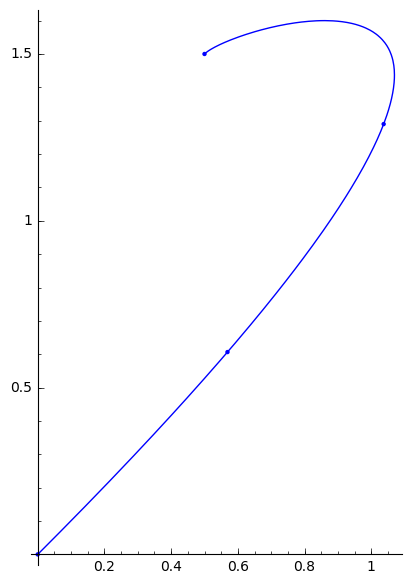
\includegraphics[scale=0.75]{4pt}
\end{center}

\vspace*{0.5cm}

Myndin með 20 jafn löng bil á $P$ er þá: \\

\begin{center}
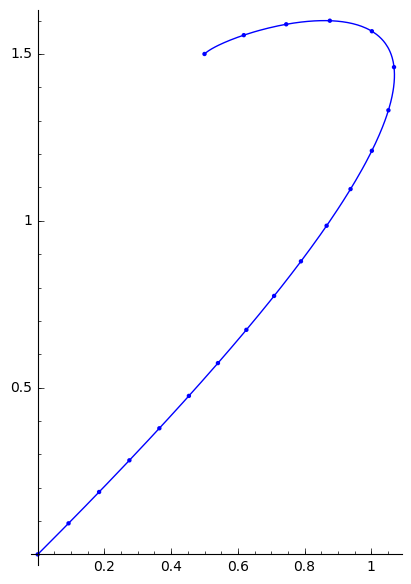
\includegraphics[scale=0.7]{20pt0}
\end{center}

\vspace*{0.5cm}

Myndin með 20 bil vigtuð með $\sqrt[3]{s}$ á $P$ er þá: \\

\begin{center}
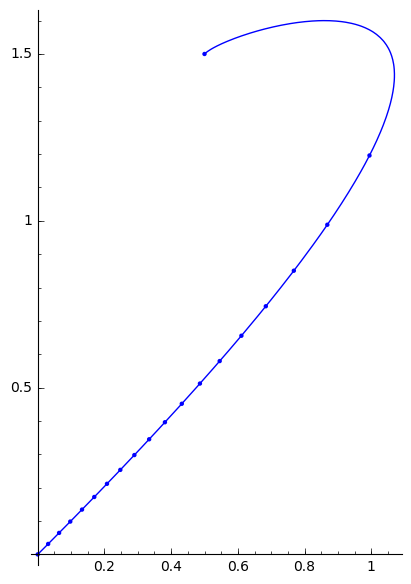
\includegraphics[scale=0.7]{20pt1}
\end{center}

\vspace*{0.5cm}

Myndin með 20 bil vigtuð með $s^2$ á $P$ er þá: \\

\begin{center}
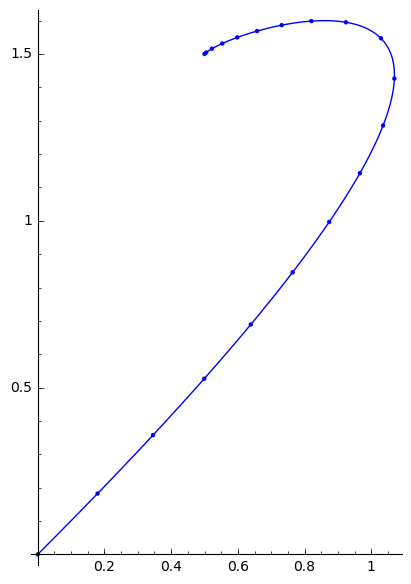
\includegraphics[scale=0.7]{20pt2}
\end{center}

\vspace*{0.5cm}

Myndin með 20 bil vigtuð með $\sin(s \pi / 2)$ á $P$ er þá: \\

\begin{center}
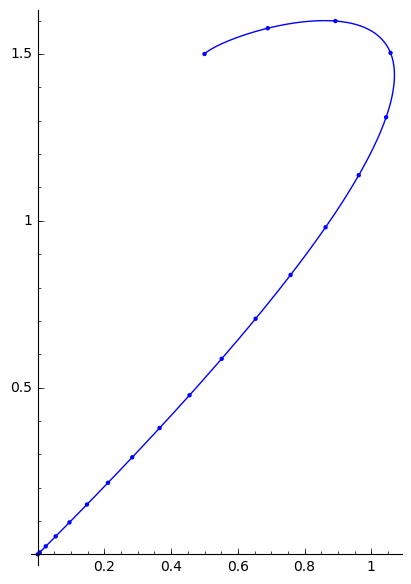
\includegraphics[scale=0.7]{20pt3}
\end{center}

\vspace*{0.5cm}

Myndin með 20 bil vigtuð með $(1 + \sin((2s - 1) \pi / 2)) / 2$ á $P$ er þá: \\

\begin{center}
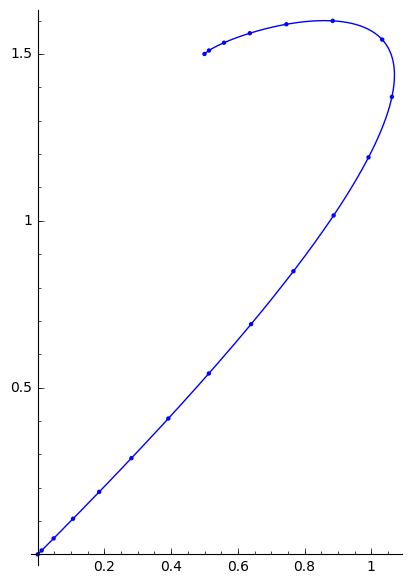
\includegraphics[scale=0.7]{20pt4}
\end{center}

\vspace*{0.5cm}

Nú næst viljum við skoða aðferð Newtons. Við þurfum þá að diffra fallið sem við vorum að finna núllstöð á, þ.e. 

\[g(x) = \int_0^x \sqrt{x'(t)^2 + y'(t)^2}dt - s\int_0^1 \sqrt{x'(t)^2 + y'(t)^2}dt = 0\]

Þar sem seinni liðurinn er fasti gefur undirstöðusetning stærðfræðigreiningarinnar að

\[g'(x) = \sqrt{x'(x)^2 + y'(x)^2} - \sqrt{x'(0)^2 + y'(0)^2}\]

Þar með gefur aðferð Newtons að ef giskið okkar er $x_n$ er næsta gisk

\[x_{n + 1} = x_n - \frac{g(x_n)}{g'(x_n)}\]

Þar sem við erum að reyna að finna punkt sem er sirka $c(s)$ hluta á leið kominn er gott gisk að byrja í $c(s)L$ þar sem $L$ er heildarlengd kúrvunnar (s.s. heildið frá 0 til 1). Helmingunarleit nálgast núllstöð línulega m.t.t. aukastafa en aðferð Newtons finnur kvaðratsfjölda aukastafa ef afleiðan í punktinum er ekki núll. Því ef $g' \neq 0$ mun Newton vera hraðari en þar sem $g' = 0$ ætti hraðinn að vera svipaður. Hins vegar er þetta háð upphafsgiski og $c$ og $x, y$ svo ekki er hægt að segja margt fleira fyrir almenn $c, x, y$. Einnig lendum við í svipuðu vandamáli og í helmingunarleit að við getum aðeins metið tolerance-inn út frá fallgildum $g$ en ekki raunverulegri fjarlægð frá rót, en að leiðbeiningum Sigurðar Freys Hafsteins þá munum við hunsa það vandamál hér. Þá má útfæra Newton eins og fylgir: \\

\begin{minted}{python}
def newtsearch(dx, dy, tol, s, c):
    alen = arclen(dx, dy, 1, tol)
    def f(x):
        return arclen(dx, dy, x, tol) - c(s) * alen
    def df(x):
        return sqrt(dx(x) ** 2 + dy(x) ** 2) - sqrt(dx(0) ** 2 - dy(0) ** 2)
    x0 = c(s) * alen
    while f(x0) > tol:
        x0 -= f(x0) / df(x0)
    return x0
\end{minted}

\vspace*{0.5cm}

TODO: Animate

TODO: Bezier

\end{document}